\documentclass[10pt]{article}
\usepackage[czech]{babel}
\usepackage[utf8]{inputenc}
\usepackage[T1]{fontenc}
\usepackage{amsmath}
\usepackage{amsfonts}
\usepackage{amssymb}
\usepackage[version=4]{mhchem}
\usepackage{stmaryrd}
\usepackage{graphicx}
\usepackage[export]{adjustbox}
\graphicspath{ {./images/} }

\title{Fyzikální praktikum 2 }


\author{Ústav fyziky kondenzovaných látek\\
Přírodovědecká fakulta, Masarykova univerzita, Brno}
\date{}


%New command to display footnote whose markers will always be hidden
\let\svthefootnote\thefootnote
\newcommand\blfootnotetext[1]{%
  \let\thefootnote\relax\footnote{#1}%
  \addtocounter{footnote}{-1}%
  \let\thefootnote\svthefootnote%
}

%Overriding the \footnotetext command to hide the marker if its value is `0`
\let\svfootnotetext\footnotetext
\renewcommand\footnotetext[2][?]{%
  \if\relax#1\relax%
    \ifnum\value{footnote}=0\blfootnotetext{#2}\else\svfootnotetext{#2}\fi%
  \else%
    \if?#1\ifnum\value{footnote}=0\blfootnotetext{#2}\else\svfootnotetext{#2}\fi%
    \else\svfootnotetext[#1]{#2}\fi%
  \fi
}

\begin{document}
\maketitle


\section*{3. Rozložení elektrického pole}
\section*{Úkoly k měření}
\section*{Rozložení potenciálu v okolí dvouvodičového vedení}
\begin{itemize}
  \item Pochopení a praktické zvládnutí měření rozložení elektrického pole v elektrolytické vaně pomocí střídavého mostu.
  \item Osvojení si schopnosti sestavení měřícího obvodu a přizpůsobení nastavení osciloskopu cílům měření.
  \item Porovnání měřeného elektrostatického pole v okolí dvouvodičového vedení s teoretickým výpočtem.
\end{itemize}

\section*{Rozložení potenciálu v okolí dvouvodičového vedení}
\section*{Teoretický úvod}
Potenciál pole ve vzdálenosti $r$ od přímého vodiče s lineární hustotou náboje $\tau$ je


\begin{equation*}
V=\frac{\tau}{2 \pi \epsilon} \ln \frac{R}{r} \tag{3.1}
\end{equation*}


kde $R$ je vzdálenost od vodiče, ve které klademe potenciál roven nule $V(R)=0$ (nelze volit $V(\infty)=0$, protože náboj je rozložen na vodiči, jehož délka není omezena). Volíme-li místo nulového potenciálu ve vzdálenosti $R=1 \mathrm{~m}$ od vodiče, pak můžeme vztah (3.1) psát


\begin{equation*}
V=-\frac{\tau}{2 \pi \epsilon} \ln r \tag{3.2}
\end{equation*}


\begin{center}
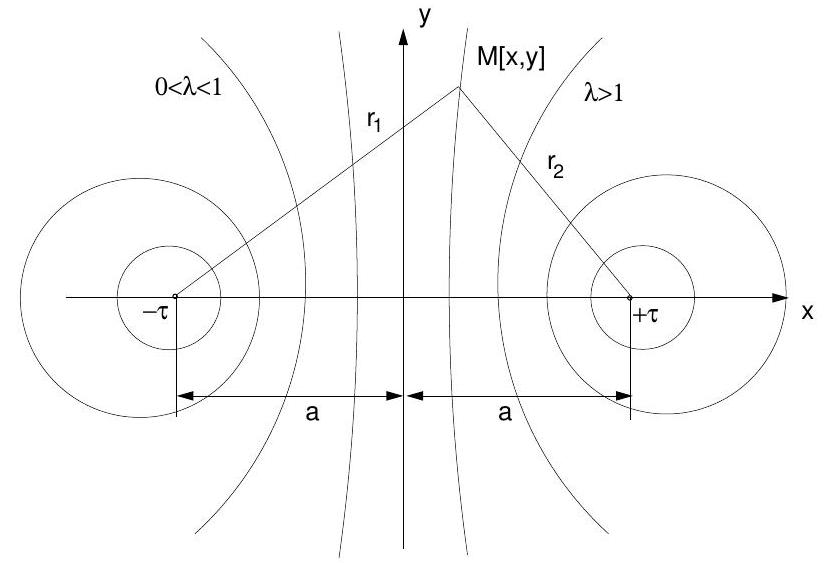
\includegraphics[max width=\textwidth]{2024_10_15_71c3161fc9161f95056eg-1}
\end{center}

Obrázek 3.1: Ekvipotenciální hladiny v rovině kolmé na dva rovnoběžné nekonečně dlouhé nabité vodiče.

Potenciál v bodě $M$ (obrázek 3.1) od dvou lineárních rovnoběžných vodičů je podle principu superpozice s přihlédnutím ke vztahu (3.2) dán


\begin{equation*}
V=V_{1}+V_{2}=\frac{\tau}{2 \pi \epsilon} \ln \frac{r_{2}}{r_{1}} \tag{3.3}
\end{equation*}


Na vodičích jsou rozloženy elektrické náboje s konstantními lineárními hustotami $+\tau$ a $-\tau$. Pro ekvipotenciály platí


\begin{equation*}
\frac{\tau}{2 \pi \epsilon} \ln \frac{r_{2}}{r_{1}}=\text { konst., } \quad \text { nebo } \quad \frac{r_{2}}{r_{1}}=\lambda \tag{3.4}
\end{equation*}


kde $r_{1}=\sqrt{(a-x)^{2}+y^{2}}, r_{2}=\sqrt{(a+x)^{2}+y^{2}}$ a $\lambda>0$ je parametr ekvipotenciálních hladin.\\
Geometrickým místem bodů v rovině, které mají od daných dvou bodů konstantní poměr vzdáleností $\lambda$, je pro $\lambda=1$ přímka a pro $\lambda \neq 1$ Apolloniova kružnice. Ve zvolené soustavě kartézských souřadnic je touto přímkou osa $y$, středy $S\left[x_{s}, 0\right]$ a poloměry $r$ Apolloniových kružnic určíme tak, že rovnice (3.4) upravíme na tvar


\begin{equation*}
\left(x-a \frac{\lambda^{2}+1}{\lambda^{2}-1}\right)^{2}+y^{2}=a^{2}\left(\frac{\lambda^{2}+1}{\lambda^{2}-1}\right)^{2}-a^{2} \tag{3.5}
\end{equation*}


Pak


\begin{equation*}
x_{s}=a \frac{\lambda^{2}+1}{\lambda^{2}-1}, \quad r=\sqrt{x_{s}^{2}-a^{2}} \tag{3.6}
\end{equation*}


Z prvních tří rovnic 3.21) plyne pro potenciál elektrostatického pole Laplaceova rovnice


\begin{equation*}
\nabla^{2} V=0 \tag{3.7}
\end{equation*}


Problém určení elektrostatického pole dvojvodičového vedení tvořeného rovnoběžnými válcovými vodiči nahradíme řešením elektrostatického pole dvojice rovnoběžných vodičů. Okrajové podmínky zachováme, postupujeme-li takto: dané válcové vodiče nahradíme válci z dielektrika s permitivitou prostředí $\epsilon$ a do každého z nich vložíme př̌ímkový vodič s lineární hustotou náboje $\tau$, resp. $-\tau$ (obrázek 3.2), tzv. elektrické osy.\\
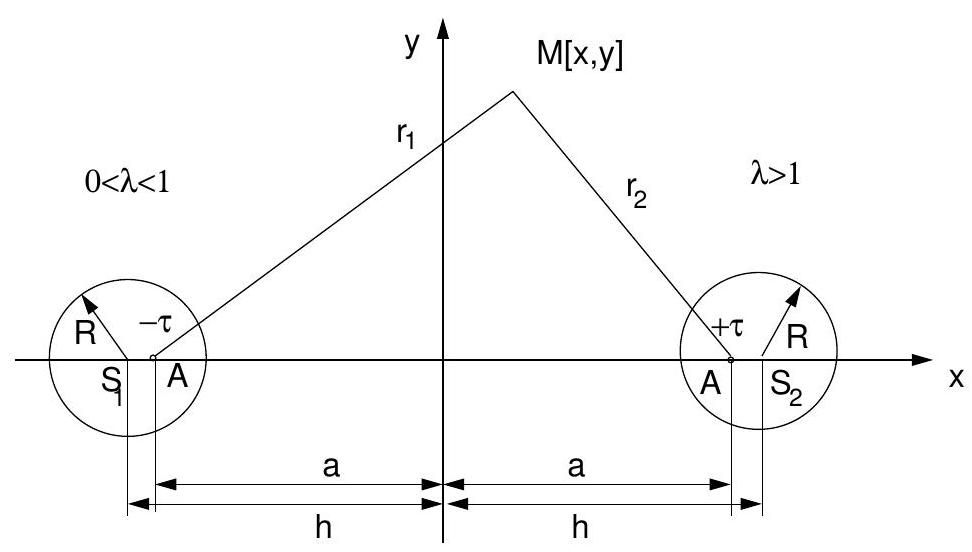
\includegraphics[max width=\textwidth, center]{2024_10_15_71c3161fc9161f95056eg-2}

Obrázek 3.2: Výpočet potenciálu v bodě $M$ od dvou válcových nekonečných vodičů s poloměrem $R$, mezi nimiž je rozdíl potenciálů $U$.

Polohu os a hodnotu $\tau$ stanovíme tak, aby elektrické pole, které vytvářejí, mělo ekvipotenciální plochy $V_{1}$ a $V_{2}$ s poloměry $R$ právě v místech povrchu válců, přičemž musí být $V_{1}-V_{2}=U$. Ve zvolené souřadné soustavě je vzdálenost středů $S_{1}$ a $S_{2}$ vodivých válců $2 h$, pak poloha náhradních vodičů $A$ a $B$ se určí z rovnice 3.6


\begin{equation*}
a=\sqrt{h^{2}-R^{2}} \tag{3.8}
\end{equation*}


Z poslední rovnice je zřejmé, že body $A$ a $B$ jsou vzájemně sdružené v kulové inverzi vzhledem ke kružnicím se středy $S_{1}$ a $S_{2}$. Pak platí


\begin{equation*}
R^{2}=h^{2}-a^{2}=(h-a)(h+a)=\overline{S_{2} A} \cdot \overline{S_{2} B}=\overline{S_{1} B} \cdot \overline{S_{1} A} \tag{3.9}
\end{equation*}


Potenciál v bodě $M$ bude podle 3.3


\begin{equation*}
V=\frac{\tau}{2 \pi \epsilon} \ln \frac{r_{2}}{r_{1}}=\frac{\tau}{2 \pi \epsilon} \ln \lambda \tag{3.10}
\end{equation*}


Pro potenciály na ekvipotenciálních plochách totožných s válcovými vodiči dostaneme podle 3.10 s použitím 3.9 .


\begin{equation*}
V_{1} \equiv \frac{\tau}{2 \pi \epsilon} \ln \frac{\overline{A P}}{\overline{B P}}=\frac{\tau}{2 \pi \epsilon} \ln \frac{h+a}{R}, \quad V_{2} \equiv \frac{\tau}{2 \pi \epsilon} \ln \frac{\overline{A Q}}{\overline{B Q}}=\frac{\tau}{2 \pi \epsilon} \ln \frac{R}{h+a} \tag{3.11}
\end{equation*}


Hodnotu $\tau$ určíme z podmínky $U=V_{1}-V_{2}$


\begin{equation*}
\tau=\frac{\pi \epsilon U}{\ln \frac{h+a}{R}} \tag{3.12}
\end{equation*}


Dosazením 3.12 do 3.10 dostaneme


\begin{equation*}
V=\frac{U}{2 \ln \frac{h+a}{R}} \ln \frac{r_{2}}{r_{1}} \tag{3.13}
\end{equation*}


Rovnice 3.10 je odvozena pro symetrické rozložení nábojů, které v běžném experimentálním uspořádání není splněno (obyčejně máme $V_{1}=U$ a $V_{2}=0$ nebo naopak a nikoliv $V_{1}=U / 2$ a $\left.V_{2}=-U / 2\right)$. Ve shodě s naším experimentálním uspořádáním posuneme hladinu, od které počítáme potenciál, o $U / 2$, tedy


\begin{equation*}
V=\frac{U}{2 \ln \frac{h+a}{R}} \ln \frac{r_{2}}{r_{1}}+\frac{U}{2} \tag{3.14}
\end{equation*}


Parametr $\lambda$ příslušející konkrétní ekvipotenciální hladině s potenciálem $V$ pak vypočteme jako


\begin{equation*}
\ln \lambda=\frac{V-\frac{U}{2}}{U} 2 \ln \frac{h+a}{R}=\left(\frac{V}{U}-\frac{1}{2}\right) 2 \ln \frac{h+a}{R} \tag{3.15}
\end{equation*}


\section*{Měření rozložení elektrostatického pole}
Elektrostatické pole je svou podstatou vektorovým polem, tvořeným vektorem intenzity $\boldsymbol{E}$. Můžeme je však stejně dobře popsat, užijeme-li skalárního pole hodnot elektrostatického potenciálu $V$. Uvedené vektorové pole intenzity a skalární pole potenciálu jsou si zcela ekvivalentní a platí


\begin{equation*}
\boldsymbol{E}=-\nabla V \tag{3.16}
\end{equation*}


Ekvipotenciální hladinou se nazývá v obecném případě plocha, na které má potenciál všude stejnou hodnotu


\begin{equation*}
V(x, y, z)=V_{0}=\text { konst } \tag{3.17}
\end{equation*}


Pro každý elementární posuv $\delta x, \delta y, \delta z$ po této ploše platí zřejmě podmínky $\delta V=0$ a tedy také


\begin{equation*}
-\left(E_{x} \delta x+E_{y} \delta y+E_{z} \delta z\right)=-\boldsymbol{E} \cdot \delta \boldsymbol{l}=0 \tag{3.18}
\end{equation*}


Tato rovnice říká, že skalární součin intenzity s libovolným posunem po hladině je nulový, tj. intenzita je všude kolmá k ekvipotenciálním hladinám a siločáry jimi probíhají kolmo.

Vztah (3.16) vede ryze matematickým postupem [1] k další důležité rovnici


\begin{equation*}
\operatorname{rot} \boldsymbol{E}=0 \tag{3.19}
\end{equation*}


tedy elektrostatické pole je pole nevírové. V místech bez náboje je také


\begin{equation*}
\operatorname{div} \boldsymbol{E}=0 \tag{3.20}
\end{equation*}


to znamená, že uvažované pole je nezřídlové.\\
Měření rozložení potenciálu v elektrostatickém poli je z experimentálního hlediska dosti obtížné. Využívá se proto analogie mezi elektrostatickým polem v homogenním dielektriku a elektrickým polem uvnitř homogenního vodiče, kterým protéká stacionární proud. V jednotlivých případech je pole popsáno:

Pole stacionárního proudu Elektrostatické pole

\[
\begin{array}{rc}
\boldsymbol{E}_{s}=-\nabla V_{s} & \boldsymbol{E}_{e}=-\nabla V_{e}  \tag{3.21}\\
\boldsymbol{j}_{s}=\sigma \boldsymbol{E}_{s} & \boldsymbol{D}_{e}=\epsilon \boldsymbol{E}_{e} \\
\operatorname{div} \boldsymbol{j}_{s}=0 & \operatorname{div} \boldsymbol{D}_{e}=0 \\
\oint \boldsymbol{E}_{s} \cdot \mathrm{~d} \boldsymbol{l}=0 & \oint \boldsymbol{E}_{e} \cdot \mathrm{~d} \boldsymbol{l}=0
\end{array}
\]

kde $\boldsymbol{E}_{s}, \boldsymbol{E}_{e}$ je vektor intenzity pole, $\boldsymbol{j}_{s}$ proudová hustota, $\boldsymbol{D}_{e}$ vektor elektrostatické indukce, $\sigma$ vodivost prostředí, ve kterém teče proud, $\epsilon$ permitivita prostředí, v němž se elektrostatické pole vyskytuje. Za předpokladu, že dielektrikum je homogenní a neexistují v něm volné náboje a vodič je homogenní $(\sigma=$ konst. $\neq 0$ ), jsou soustavy rovnic 3.21 pro pole stacionárního proudu a elektrostatické pole zcela ekvivalentní. Pak lze elektrostatické pole trojrozměrného systému v prostředí s permitivitou $\epsilon$ studovat jako pole proudu $\boldsymbol{j}_{s} \mathrm{v}$ prostředí s vodivostí $\sigma$. Měření obyčejně provádíme v rovině, tj. studujeme takové trojrozměrné systémy, které mohou být popsány rozložením pole v určité rovině. Jsou to jednak systémy nezávislé na jedné ze souřadných os a jednak systémy, které mají rotační symetrii. Poslední případ se týká např. elektrostatických čoček.

\section*{Střídavý můstek}
Střídavý most zahrnuje čtyři impedance zapojené dle obrázku 3.3 (vlevo). Most je vyvážen tehdy, jestliže detektorem $D$ neprochází proud, pak jsou splněny jisté relace mezi impedancemi v jednotlivých větvích mostu. V případě střídavého mostu je situace poněkud komplikovanější ve srovnání se stejnosměrným mostem, protože na impedancích dochází obecně k fázovému posuvu proudu a napětí. Napětí na jednotlivých impedancích je rovno $\hat{U}_{i}=\hat{Z}_{i} \hat{I}_{i}$, tedy

\[
\begin{array}{ll}
\hat{U}_{1}=\hat{Z}_{1} \hat{I}_{1}, & \hat{U}_{2}=\hat{Z}_{2} \hat{I}_{2} \\
\hat{U}_{3}=\hat{Z}_{3} \hat{I}_{3}, & \hat{U}_{4}=\hat{Z}_{4} \hat{I}_{4} \tag{3.22}
\end{array}
\]

Jestliže detektorem neprochází proud, je $\hat{I}_{D}=0$ a platí $\hat{I}_{1}=\hat{I}_{2}, \hat{I}_{3}=\hat{I}_{4}$ a

\[
\begin{array}{ll}
\hat{U}_{1}=\hat{Z}_{1} \hat{I}_{1}, & \hat{U}_{2}=\hat{Z}_{2} \hat{I}_{1} \\
\hat{U}_{3}=\hat{Z}_{3} \hat{I}_{3}, & \hat{U}_{4}=\hat{Z}_{4} \hat{I}_{3} \tag{3.23}
\end{array}
\]

a současně je zřejmé, že $\hat{U}_{B D}=0$. Tedy musí platit $\hat{U}_{1}=\hat{U}_{3}$ a $\hat{U}_{2}=\hat{U}_{4}$. Pak dostaneme obecnou podmínku rovnováhy na střídavém mostě


\begin{equation*}
\frac{\hat{Z}_{1}}{\hat{Z}_{2}}=\frac{\hat{Z}_{3}}{\hat{Z}_{4}} \tag{3.24}
\end{equation*}


Tato podmínka představuje vlastně dvě rovnice, pro reálnou a imaginární část impedancí $\hat{Z}_{i}$. Jestliže vyjádříme impedanci $\hat{Z}$ ve tvaru


\begin{equation*}
\hat{Z}=|\hat{Z}| \mathrm{e}^{\mathrm{i} \phi} \tag{3.25}
\end{equation*}


kde $|\hat{Z}|$ je absolutní hodnota a $\phi$ fázový posuv, dostaneme ze vztahu 3.24 amplitudovou podmínku


\begin{equation*}
\frac{\left|\hat{Z}_{1}\right|}{\left|\hat{Z}_{2}\right|}=\frac{\left|\hat{Z}_{3}\right|}{\left|\hat{Z}_{4}\right|} \tag{3.26}
\end{equation*}


a podmínku fázovou


\begin{equation*}
\phi_{1}-\phi_{2}=\phi_{3}-\phi_{4}+2 k \pi, \quad k=0,1,2, \ldots \tag{3.27}
\end{equation*}


Aby byl střídavý most vyvážen, musí být obě podmínky splněny současně.

\section*{Postup měření:}
Měření se provádí v elektrolytické vaně zapojené jako střídavý můstek. Je to nevodivá nádoba se slabým elektrolytem, do níž se umístí modely vodičù, jejichž elektrické pole chceme vyšetřovat. Rozměry nádoby je nutno volit tak, aby hustota proudu u jejich stěn byla mnohem menší než v prostoru, kde měříme. Na obrázku 3.3 je schéma zapojení vany do střídavého mostu se dvěma elektrodami $M_{1}$ a $M_{2}$. Oba kanály osciloskopu jsou připojeny k obvodu pomocí koaxiálních kabelů, jejichž stínící vodiče propojují zemněný vodič generátoru se zemí osciloskopu. Sondou (S) je kovová jehla sloužící k mapování potenciálu ve vaně. Sonda je připevněna k pantografu přes nějž je poloha jehly přenášena do grafického tabletu a z něj do měřícího programu běžícího na PC. Dále je sonda spojena s kanálem 1 osciloskopu. Kanál 2 osciloskopu je připojen k jezdci potenciometru, pomocí něhož nastavujeme referenční potenciál. Osciloskop je pak nastaven v režimu měření rozdílu signálů na kanálech $1 \mathrm{a} 2, \mathrm{tj} .{ }_{1}-2$. Nastavený potenciálový rozdíl mezi zemí obvodu a jezdcem potenciometru je měřen pomocí voltmetru.

Sondou $S$ hledáme ta místa v elektrolytu, jejichž potenciál je stejný jako potenciál $U_{1}$ nastavený na potenciometru $\left(S_{1}\right)$. Je-li potenciál sondy a jezdce potenciometru stejný, pak osciloskop vykazuje minimální signál. To odpovídá přibližně rovné čáře na osciloskopu.

Pomocí odečítacího zařízení (pantografu) lze postupně přes grafický tablet přenést do ovládacího programu na PC sít bodů o stejném potenciálu. Jejich spojením dostáváme průběh ekvipotenciální čáry. Siločáry jsou v každém bodě kolmé k ekvipotenciálním čarám: takovým způsobem lze postupně zmapovat průběh elektrostatického pole v určité rovině.\\
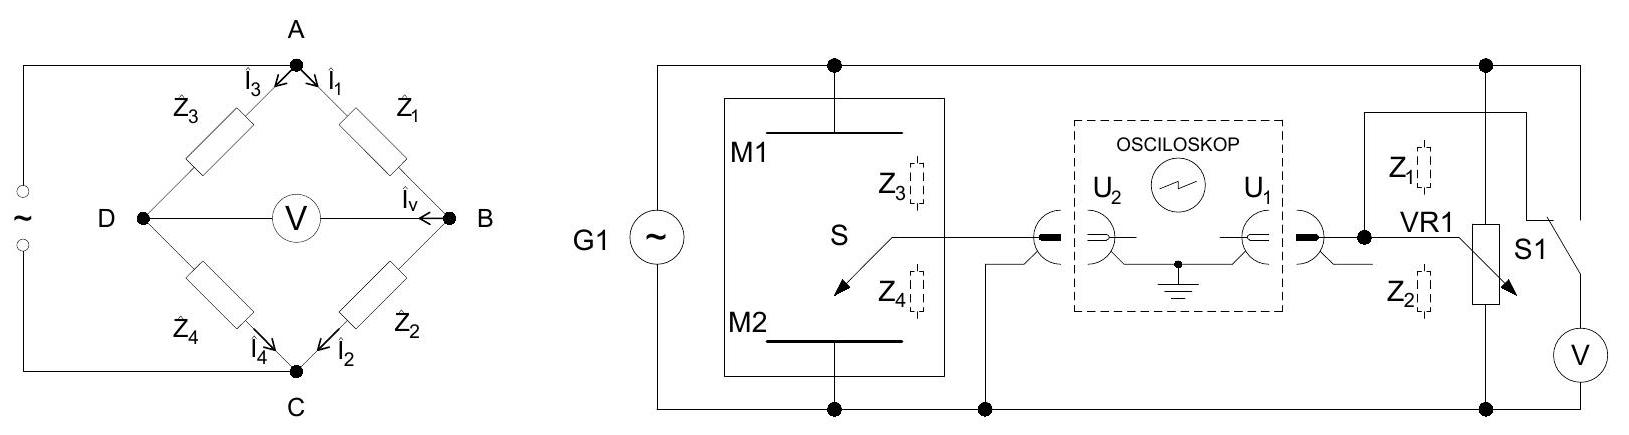
\includegraphics[max width=\textwidth, center]{2024_10_15_71c3161fc9161f95056eg-5}

Obrázek 3.3: Obecný střídavý můstek (vlevo). Zapojení střídavého můstku pro měření v elektrolytické vaně (vpravo) se zakreslenými ekvivalenty impedancí v levém obrázku (čerchovaně zakreslené značky rezistoru). Osciloskop je k obvodu připojen přes koaxiální kabely, jejichž stínící vodiče propojují zemněný vodič generátoru se zemí osciloskopu.

Měření zpravidla provádíme střídavým proudem. Vyhneme se tím možné chybě způsobené polarizací elektrod 3]. Je-li frekvence střídavého proudu $10^{2}$ až $10^{3} \mathrm{~Hz}$, pracujeme v podstatě s kvazistacionárními proudy a ekvivalentnost systému rovnic 3.21 je splněna v tomto případě

\footnotetext{${ }^{0}$ Signální kontakty kabeláže jak na osciloskopu tak na funkčním generátoru mají červenou barvu, kdežto stínící (uzemněné) kontakty bud' modrou nebo černou barvu.
}
s dostatečnou přesností. Popsaná metoda je již poněkud překonaná moderními metodami, poskytuje však velmi dobrou představu o průběhu ekvipotenciálních čar v sestavené konfiguraci. Je-li napětí na elektrodách $\sim 10 \mathrm{~V}$ a detektorem lze měřit změny napětí řádově $10^{-2} \mathrm{~V}$, určíme polohu ekvipotenciálních čar s přesností asi $1 \%$ [2].

\section*{Úkoly}
\begin{enumerate}
  \item Určete rozložení ekvipotenciálních čar v okolí dvouvodičového vedení tvořeného rovnoběžnými válcovými vodiči.
  \item Ověřte výpočtem experimentálně získané rozložení ekvipotenciálních čar. Jednak vypočtěte parametry Apolloniových kružnic $\lambda, x_{\mathrm{s}}$ a $r$ (viz obr. 3.2 a 3.5, 3.6, 3.8 a 3.15) odpovídajících jednotlivým měřeným ekvipotenciálním hladinám a uved’te je do tabulky v protokolu. Dále pak zakreslete takto určené teoretické ekvipotenciální čáry do grafu s ekvipotenciálami naměřenými. ${ }^{1}$
\end{enumerate}

\section*{Literatura k úloze 3}
[1] Z. Horák, F. Krupka: Fyzika, SNTL Praha (1976).\\
[2] J. Brož a kol.: Základy fyzikálních měření I, SPN Praha (1983).\\
[3] V. Petržílka, S. Šafrata: Elektřina a magnetismus, NČSAV Praha (1956).\\
[4] V. Votruba, Č. Muzikář: Teorie elektromagnetického pole, NČSAV Praha (1955).

\footnotetext{${ }^{1} \mathrm{~K}$ zobrazení naměřených a vypočtených průběhů ekvipotenciálních hladin lze s výhodou použít programovacích jazyků jako Python, Octave či Matlab; softwaru jako Gnuplot nebo QtiPlot; on-line nástrojů typu GeoGebra či Desmos.
}
\end{document}